\documentclass[11pt, oneside]{article}   	% use "amsart" instead of "article" for AMSLaTeX format
\usepackage{geometry}                		% See geometry.pdf to learn the layout options. There are lots.
\geometry{letterpaper}                   		% ... or a4paper or a5paper or ... 
%\geometry{landscape}                		% Activate for rotated page geometry
%\usepackage[parfill]{parskip}    		% Activate to begin paragraphs with an empty line rather than an indent
\usepackage{graphicx}				% Use pdf, png, jpg, or eps§ with pdflatex; use eps in DVI mode
								% TeX will automatically convert eps --> pdf in pdflatex		
\usepackage{amssymb}

%SetFonts

%SetFonts


\title{An updated proposal of J-PARC T59 experiment\\
A test experiment to develop a 3D grid-like neutrino detector
with a water target for measurement of neutrino cross sections
at the near detector hall of J-PARC neutrino beam-line}
\author{The Author}
%\date{}							% Activate to display a given date or no date

\begin{document}
\maketitle

\section{Motivation}
The T2K (Tokai-to-Kamioka) experiment is a long baseline neutrino oscillation experiment.
In 2013, T2K made the first observation of electron neutrino appearance in a muon neutrino beam
with a $7.3\sigma$ significance and constrained the CP violating phase $\delta_{CP}$ based on
a data set corresponding to $8.4\%$ of the approved delivered Protons On Target (POT) \cite{t2k_nue_appearance_2013}.
In 2016, T2K indicated the CP violation with $90\%$ confidence level based on
a data set corresponding to $20\%$ of the approved delivered POT\cite{t2k_cp_2016}.
T2K is increasing its POT toward for the discovery of the CP violation.


T2K uses Super-Kamiokande (SK) as the far detector to measure neutrino interactions
at a distance of 295 km from the accelerator, and near detectors at J-PARC.
The near detectors consist of an on-axis Interactive Neutrino Grid detector (INGRID)
and an off-axis detector, ND280.
Uncertainties on neutrino flux and cross sections for T2K oscillation analyses are largely constrained
by ND280 measurement.
However, some part of systematic errors for neutrino cross sections cannot be fully constrained by the ND280 measurement because of its limited angular acceptance for the charged particle tracks.
The uncertainty (rms/mean in \%) on the predicted number of signal $\nu_{e}$ events for each group
of systematic uncertainties in the T2K oscillation analysis \cite{t2K_cp_2016} is shown in Table \ref{table:t2k_error_2016}.
In order to fully exploit the statistical power, there is an urgent need to reduce the neutrino cross section errors.


In the test experiment, we will develop a new neutrino detector, WAGASCI (WAter Grid And SCIntillator detector), to measure neutrino cross sections
on water and hydrocarbon targets with high precision and large angular acceptance.
A new idea, a 3D grid-like structure of scintillator bars, is adopted to detect tracks of charged particles
with $4\pi$ angular acceptance and larger mass ratio of water to scintillator bars.
The goal of the test experiment is to test the basic performance of the detector,
such as track reconstruction efficiency and particle identification capability using neutrino beam data,
and confirm the capability of measuring the cross section.
In order to achieve the goal, we would like to use the B2 floor of the near detector hall of J-PARC neutrino beam-line as a test facility of the neutrino beam.
We request $X \times 10^{21} POT$ of $\nu$ (not anti-$\nu$) beam with the full detector configuration.

\section{Experimental method}
Fig. \ref{fig:t59_detectors} shows a schematic view of the entire set of detectors.
Two central detectors, WAGASCI modules, contain the neutrino target material, water, and plastic scintillator bars,
and are placed along the beam direction.
The muon range detectors (MRDs) consist of two detectors in the side region (side-MRD modules)
and one detector in the downstream region (downstream-MRD) around the central detector.

\begin{figure}%[htbp]
  \begin{center}
  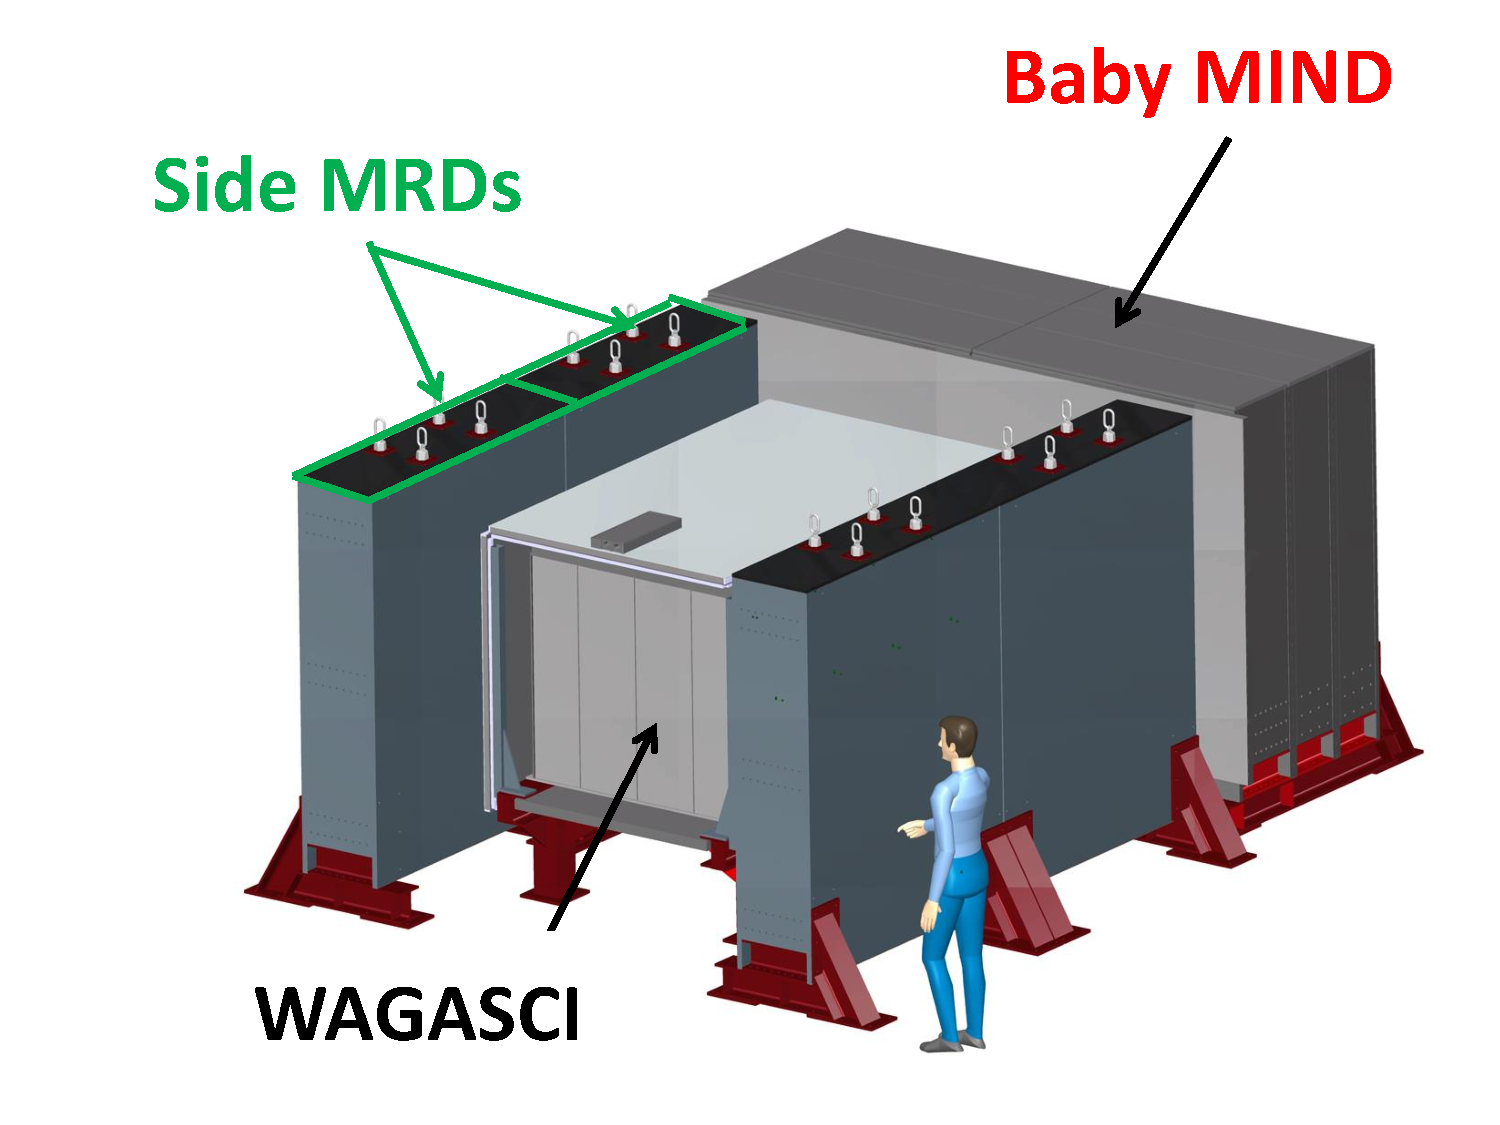
\includegraphics[width=0.6\textwidth]{figs/t59_detectors.pdf}
  \caption{Schematic view of the entire set of detectors.}
  \label{fig:t59_detectors}
  \end{center}
\end{figure}


\subsection{WAGASCI modules}
The dimension of neutrino target region in one WAGASCI module is 
100cm $\times$ 100cm in the x and y directions and 50cm along the beam direction.
The total water mass serving as neutrino target is $\sim$400kg per each module (the remaining $\sim$ 100kg is the plastic scintillator mass).
Inside the WAGASCI modules, plastic scintillator bars are aligned as a 3D grid-like structure,
shown in Fig. \ref{fig:3d_grid_structure}, and spaces in the structure are filled with water.
When neutrinos interact with hydrogen and oxygen in water, charged particles are generated.
Neutrino interactions are identified by detecting tracks of charged particles through plastic scintillator bars.
Thanks to the 3D grid-like structure of the scintillator bars,
the WAGASCI modules have $4\pi$ angular acceptance for charged particles.
Thin plastic scintillator bars (thickness $\sim$ 0.3cm) are used for the WAGASCI modules
to reduce the mass ratio of scintillator bars to neutrino target materials,
because neutrino interactions in the scintillator bars are a background for the cross section measurements.
Scintillator bars whose dimensions are 2.5cm $\times$ 0.3cm $\times$ 100cm are used for the WAGASCI modules.
The total number of channels in the two WAGASCI modules is 1280.

\begin{figure}%[htbp]
  \begin{center}
  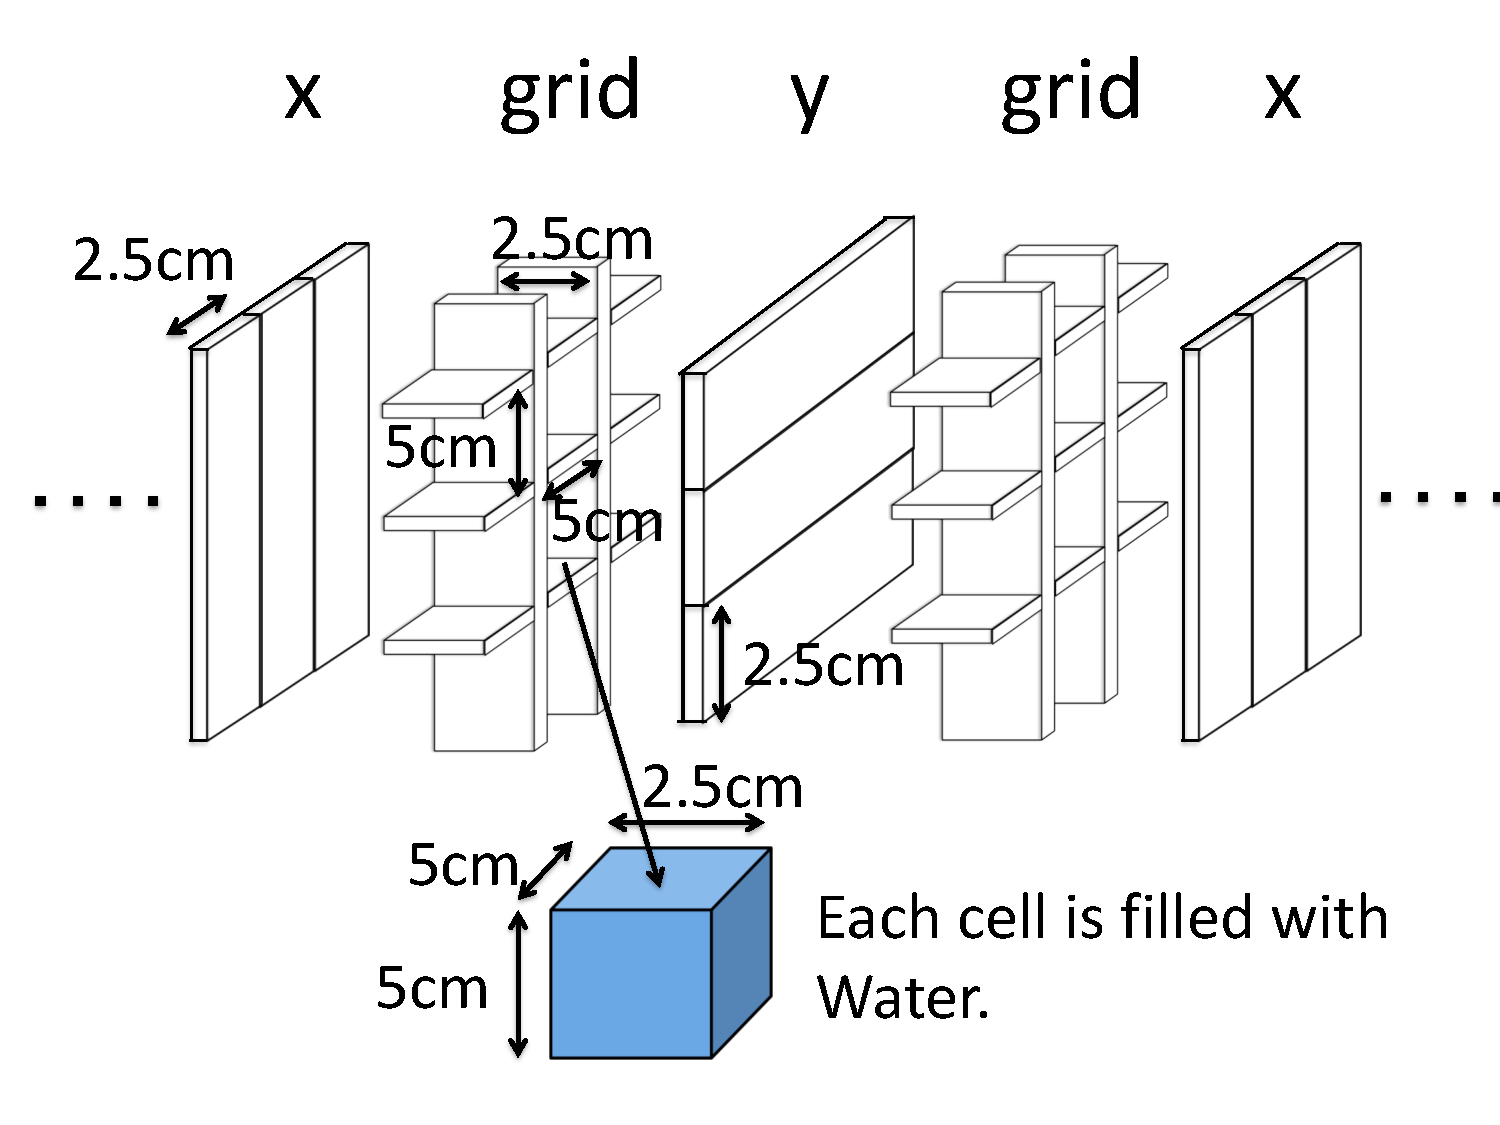
\includegraphics[width=0.6\textwidth]{figs/3d_grid_structure.pdf}
  \caption{Schematic view of 3D grid-like structure of plastic scintillator bars inside the WAGASCI module.}
  \label{fig:3d_grid_structure}
  \end{center}
\end{figure}


\subsection{Side-MRD modules}
The dimension of one side-MRD module is 161cm(width) $\times$ 180cm(height) 
in a plane along the beam direction and 46cm perpendicular to the beam direction.
The module consists of 11 3cm thick iron plates and 10 tracking scintillator planes.
Each tracking scintillator layer of the module has 8 scintillator bars whose dimensions are
20cm(width) $\times$ 0.7cm(thickness) $\times$ 180cm(length) making a plane measuring $160\times180$cm$^{2}$
in the horizontal and vertical directions.
The total number of channels in two side-MRD modules is 160.
The mechanical drawings of the side MRD are shown in Fig. \ref{fig:mec_drawing_side_mrd}.
The total weight of one side-MRD module is less than 10 ton, and it can be moved to the B2 floor using the crane in the NM pit.
The role of the side-MRD modules is the selection of muon tracks from the charged-current (CC) interactions and the rejection of short tracks caused by neutral particles, neutron and gammas,
that originate mainly from neutrino interactions in material surrounding the WAGASCI modules,
like the wall of the detector hall, or neutral-current (NC) interactions.
The muon momentum can be reconstructed from its range inside the module.
The side-MRD modules are located 50cm away from the WAGASCI modules to identify the 
direction of motion of charged particles from the hit-time difference between the two detectors,
and reject charged-particle background that originates from neutrino interactions
in the material surrounding the WAGASCI modules, like the hall of the detector hall and the side-MRD modules themselves.

\begin{figure}%[htbp]
  \begin{center}
  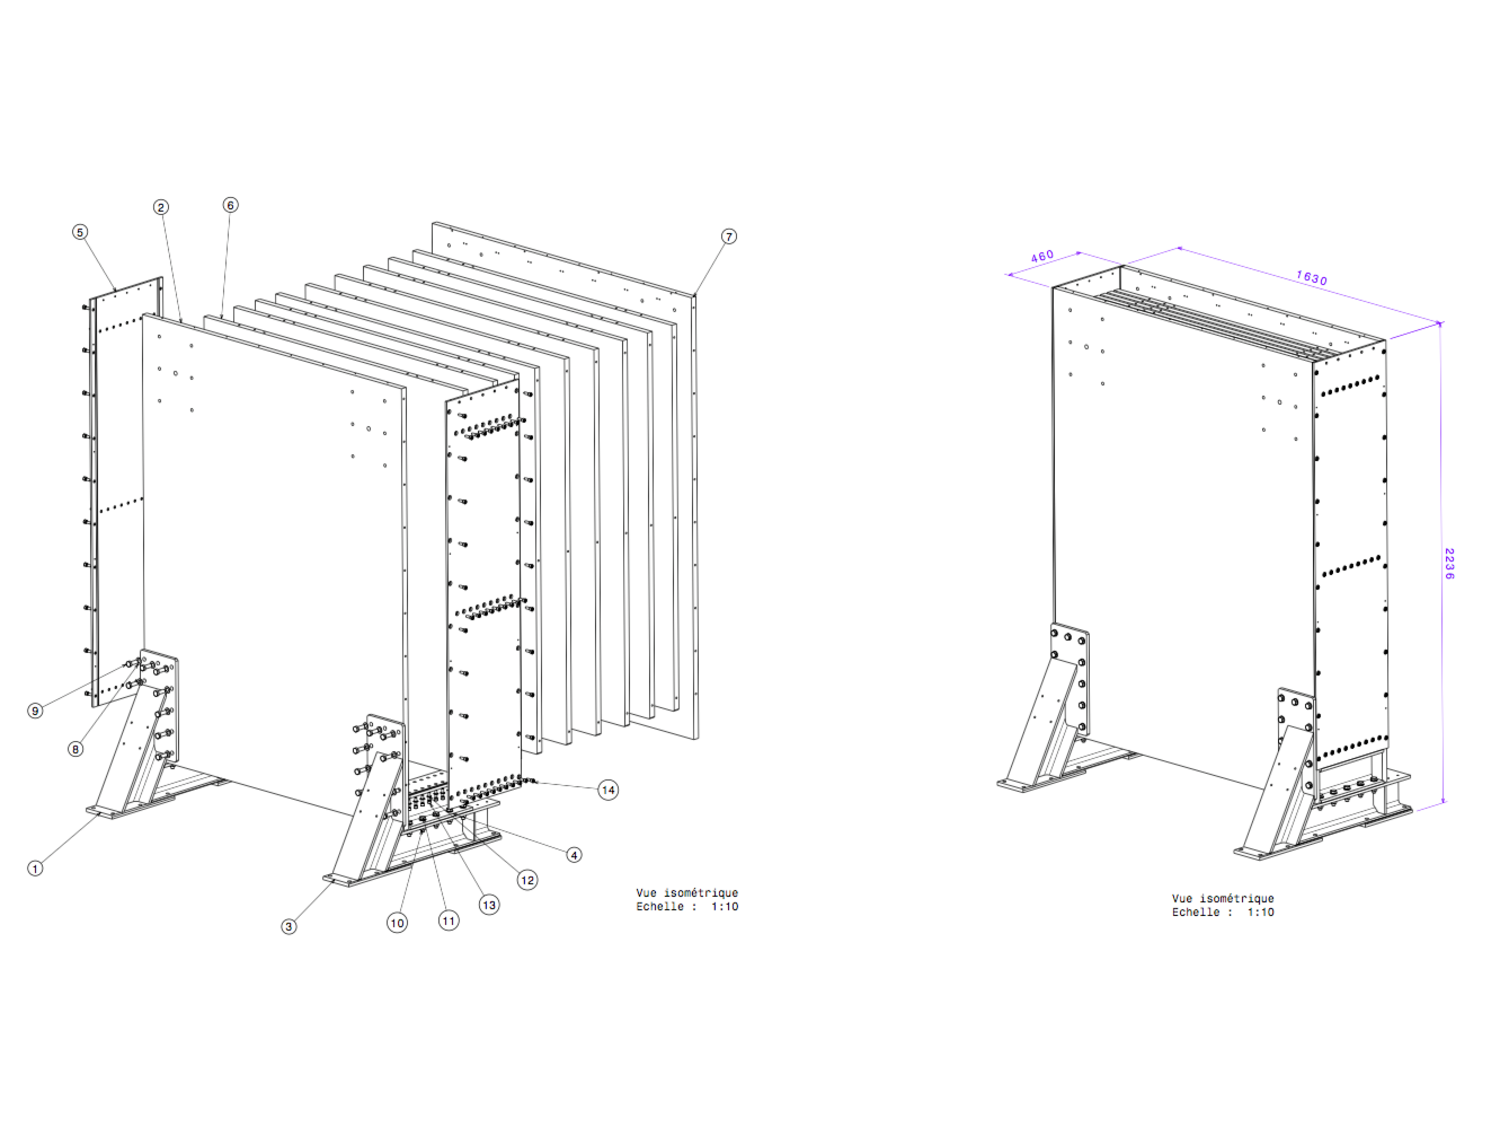
\includegraphics[width=0.8\textwidth]{figs/mec_drawing_side_mrd.pdf}
  \caption{Mechanical drawings of the side-MRD module.}
  \label{fig:med_drawing_side_mrd}
  \end{center}
\end{figure}


\subsection{BabyMIND}
As for the downstream-MRD, there is an update from the original proposal.
We have decided to magnetize the downstream MRD to realize high charge identification efficiencies for $\mu^{+}$/$\mu^{-}$ down to 500 MeV/c,
and the Baby-MIND\cite{BabyMIND} is used as the downstream-MRD.
The Baby-MIND experiment is the approved project by the CERN Research Board in December 2015,
and the Baby-MIND is the magnetized MRD developed in the experiment.
The dimension of the Baby-MIND is 350cm(width) $\times$ 200cm(height) 
in a plane perpendicular to the beam direction and 451cm along the beam direction.
% 33x5 + 19x4 + 200+10 = 451cm
The module consists of 33 5cm-thick steel magnet modules and 19 4cm-thick scintillator detector modules.
Fig. \ref{fig:baby_mind_layout} shows the layout of the Baby-MIND.


\begin{figure}%[htbp]
  \begin{center}
  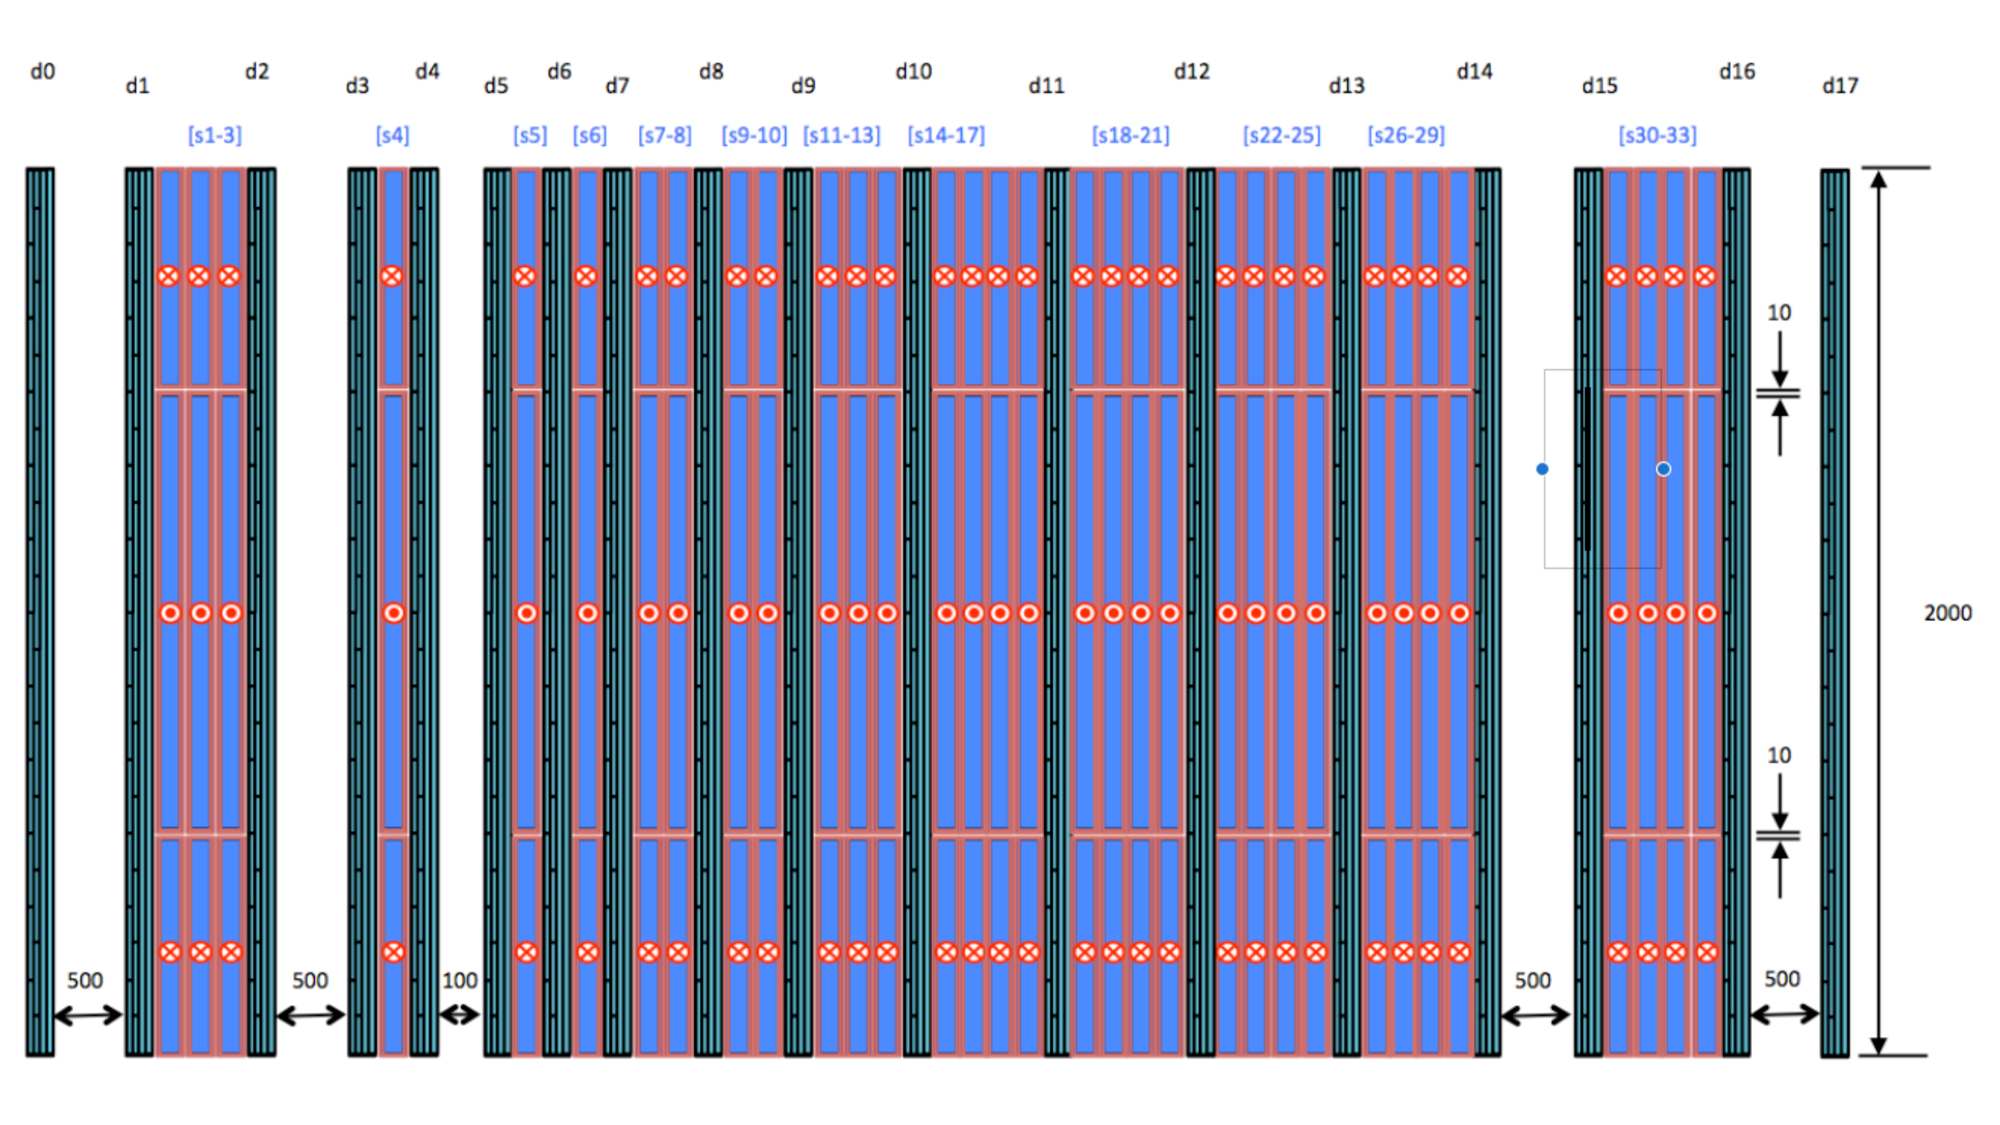
\includegraphics[width=0.8\textwidth]{figs/baby_mind_layout.pdf}
  \caption{Layout of the Baby-MIND. Muons incident from the left. 
  Steel magnet modules are shown as s1 to s33, and scintillator detector modules are shown as d0 to d17.}
  \label{fig:baby_mind_layout}
  \end{center}
\end{figure}


\subsubsection{Magnet modules}
Dimensions of each magnet module are length 350cm, height 200cm, thickness 5cm,
and its weight is 1900 kg.


The magnetic flux was measured to be very uniform over the central tracking region
from simulations as shown in Fig. \ref{fig:mag_simulation_baby_mind}.
This was confirmed by measuring the field with 9 pick-up coils wound around the first module.
All 33 modules achieve the required field of 1.5T for a current of 140 A.

\begin{figure}%[htbp]
  \begin{center}
  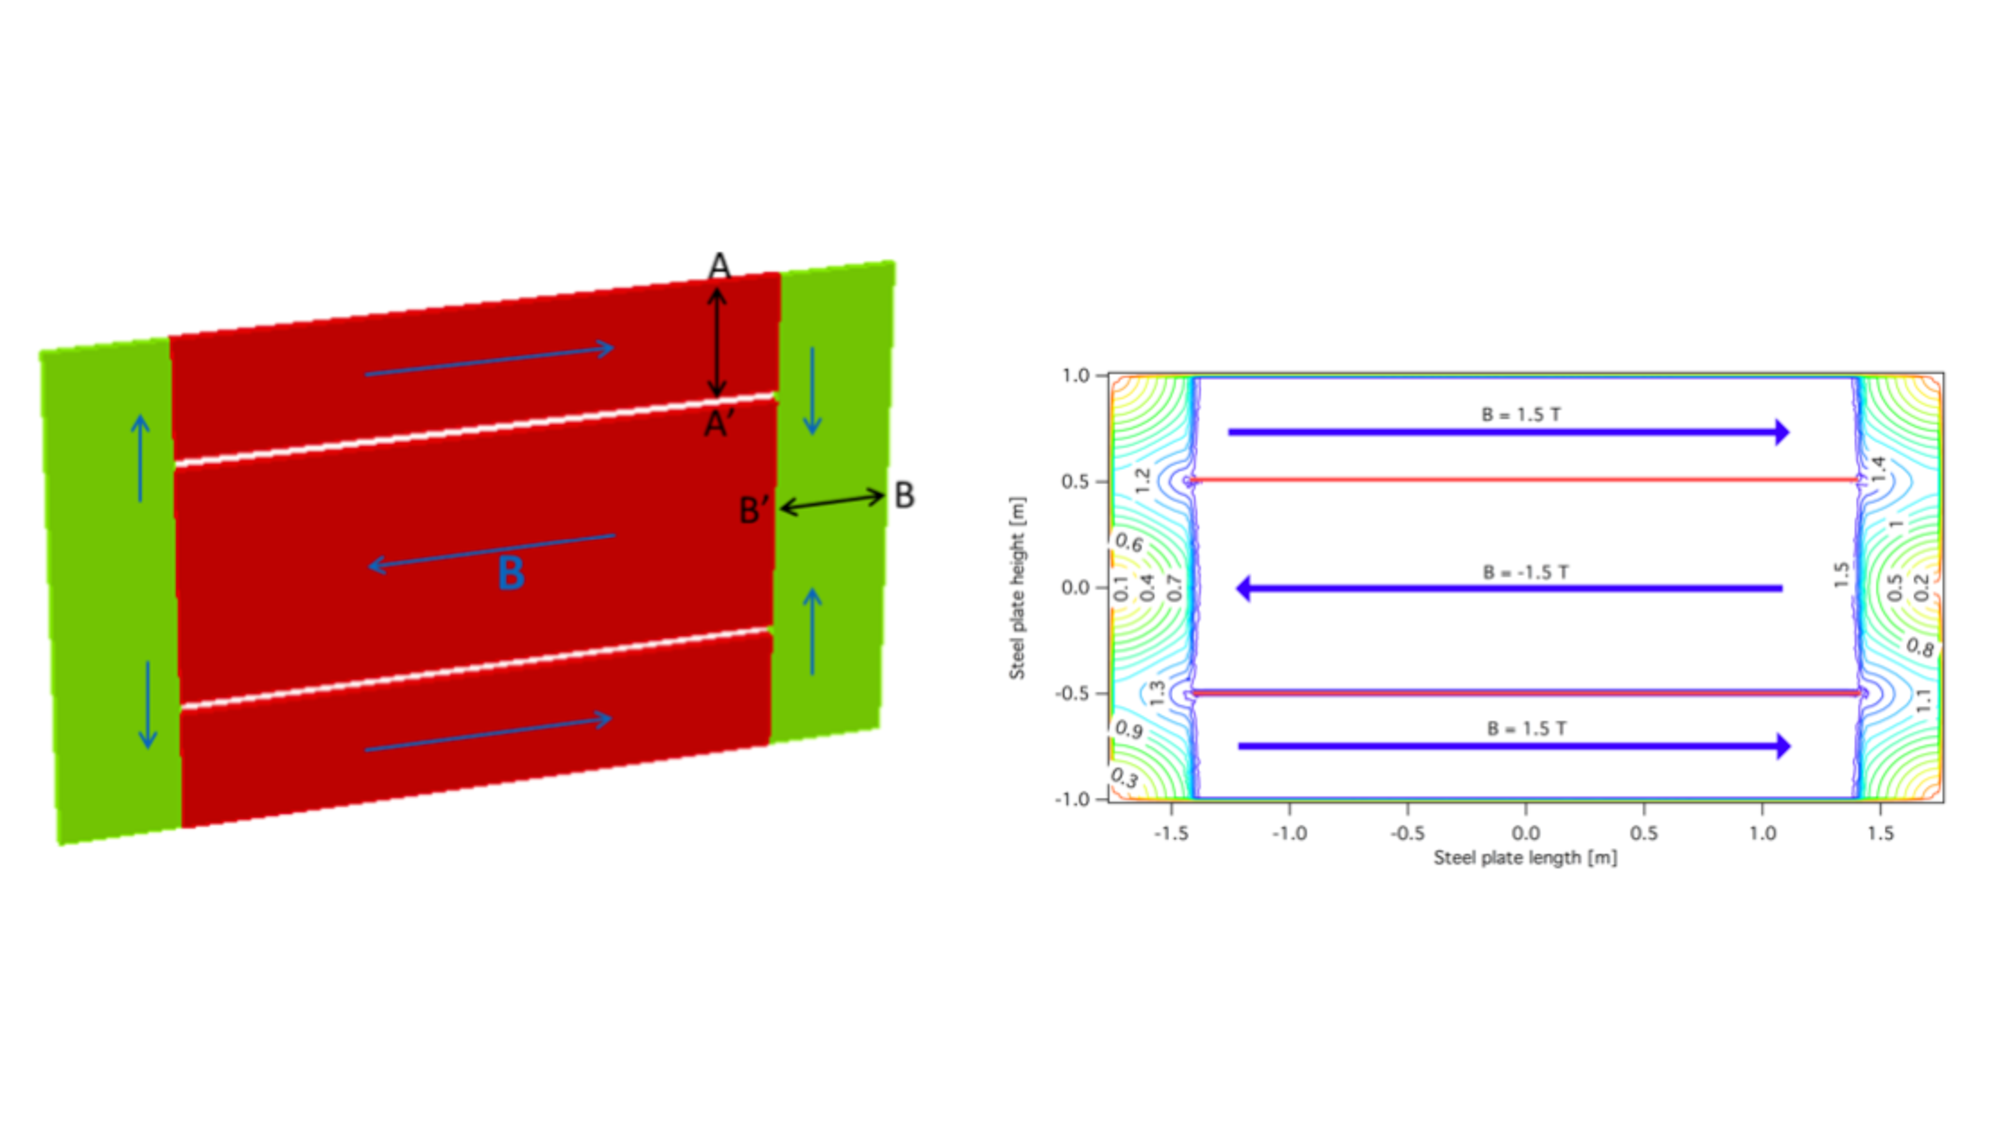
\includegraphics[width=1.0\textwidth]{figs/mag_simulation_baby_mind.pdf}
  \caption{Complete return of the magnetic flux requires cross-sections A-A' and B-B' to be equal (Left figure). Magnetic field map with a 280cm long coil, 1.5kA (Right figure).}
  \label{fig:mag_simulation_baby_mind}
  \end{center}
\end{figure}


The total power consumption for 33 magnet modules is 12 kW.
This is derived from the coil resistance inferred from the voltage drop across the power supply.
Two power supplies have been purchased to power the Baby MIND magnet,
compatible with operation both in CERN and in Japan.


\subsubsection{Scintillator detector modules}
A half of scintillator detector modules has 8 vertical scintillator bars
(dimensions: 195cm $\times$ 21cm $\times$ 0.7cm)
and 95 horizontal bars (dimensions: 290 cm x 3 cm x 0.7cm).
Each half-module is assembled independently, then coupled to its corresponding half-module
to form a complete module, \ref{fig:scinti_layer_baby_mind}.
The weight of each scintillator detector module is 300 kg.

\begin{figure}%[htbp]
  \begin{center}
  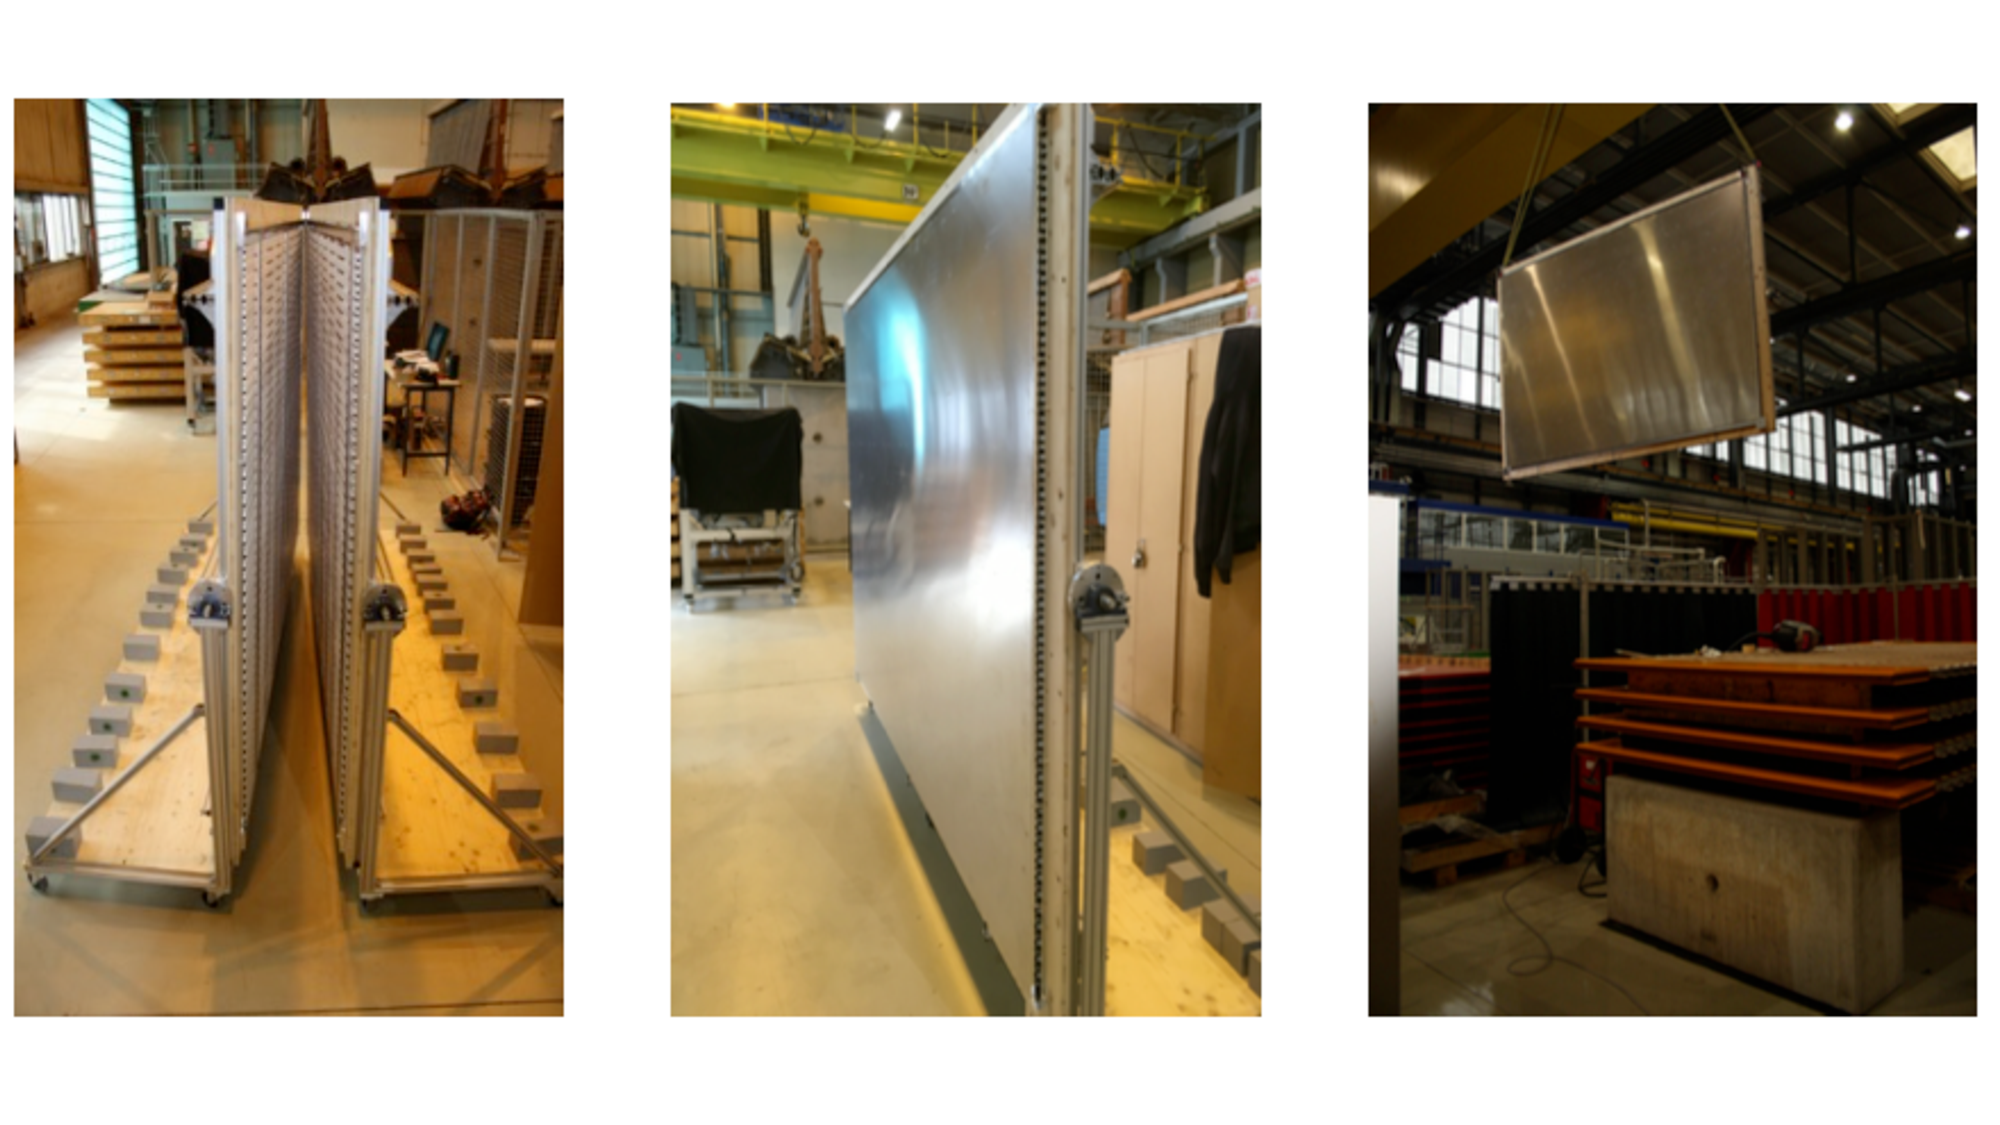
\includegraphics[width=0.8\textwidth]{figs/scinti_layer_baby_mind.pdf}
  \caption{One scintillator detector module consists of two half-modules.}
  \label{fig:scinti_layer_baby_mind}
  \end{center}
\end{figure}



\subsection{Scintillation light measurement and readout electronics}
Scintillation light in the scintillator bar of the WAGASCI modules, the side-MRD modules and Baby-MIND is collected and transported to a photodetector with a wavelength shifting fiber (WLS fiber).
The light is read out by a photodetector, Multi-Pixel Photon Counter (MPPC), attached the 
WLS fiber.
One-side readout is adapted for the WAGASCI modules,
and two-side readout is adapted for the side-MRD modules and Baby-MIND.
The signal from the MPPC is read out by the dedicated electronics developed for the test experiment
to enable bunch separation in the beam spill.
The readout electronics is triggered using the beam-timing signal from J-PARC MR to synchronize to the beam.
The beam-timing signal is branched from those for T2K, and will not cause any effect on the T2K data taking.


\subsection{Candidate experimental site}
T2K is adopting the off-axis beam method, in which the neutrino beam is directed 2.5 degrees
away from SK producing a narrowband $\nu_{\mu}$ beam.
The off-axis near detector, ND280, is installed towards the SK direction in the B1 floor of the near detector hall of the J-PARC neutrino beamline.
We are planning to install our detector in the B2 floor of the near detector hall,
where the off-axis angle is similar, and therefore an energy spectrum similar to ND280 and SK is expected.
The candidate detector position in the B2 floor is shown in Fig. \ref{fig:detector_position_b2}.
The expected neutrino energy spectrum at the candidate position is shown in Fig. \ref{fig:nu_flux_b2}.

\begin{figure}%[htbp]
  \begin{center}
  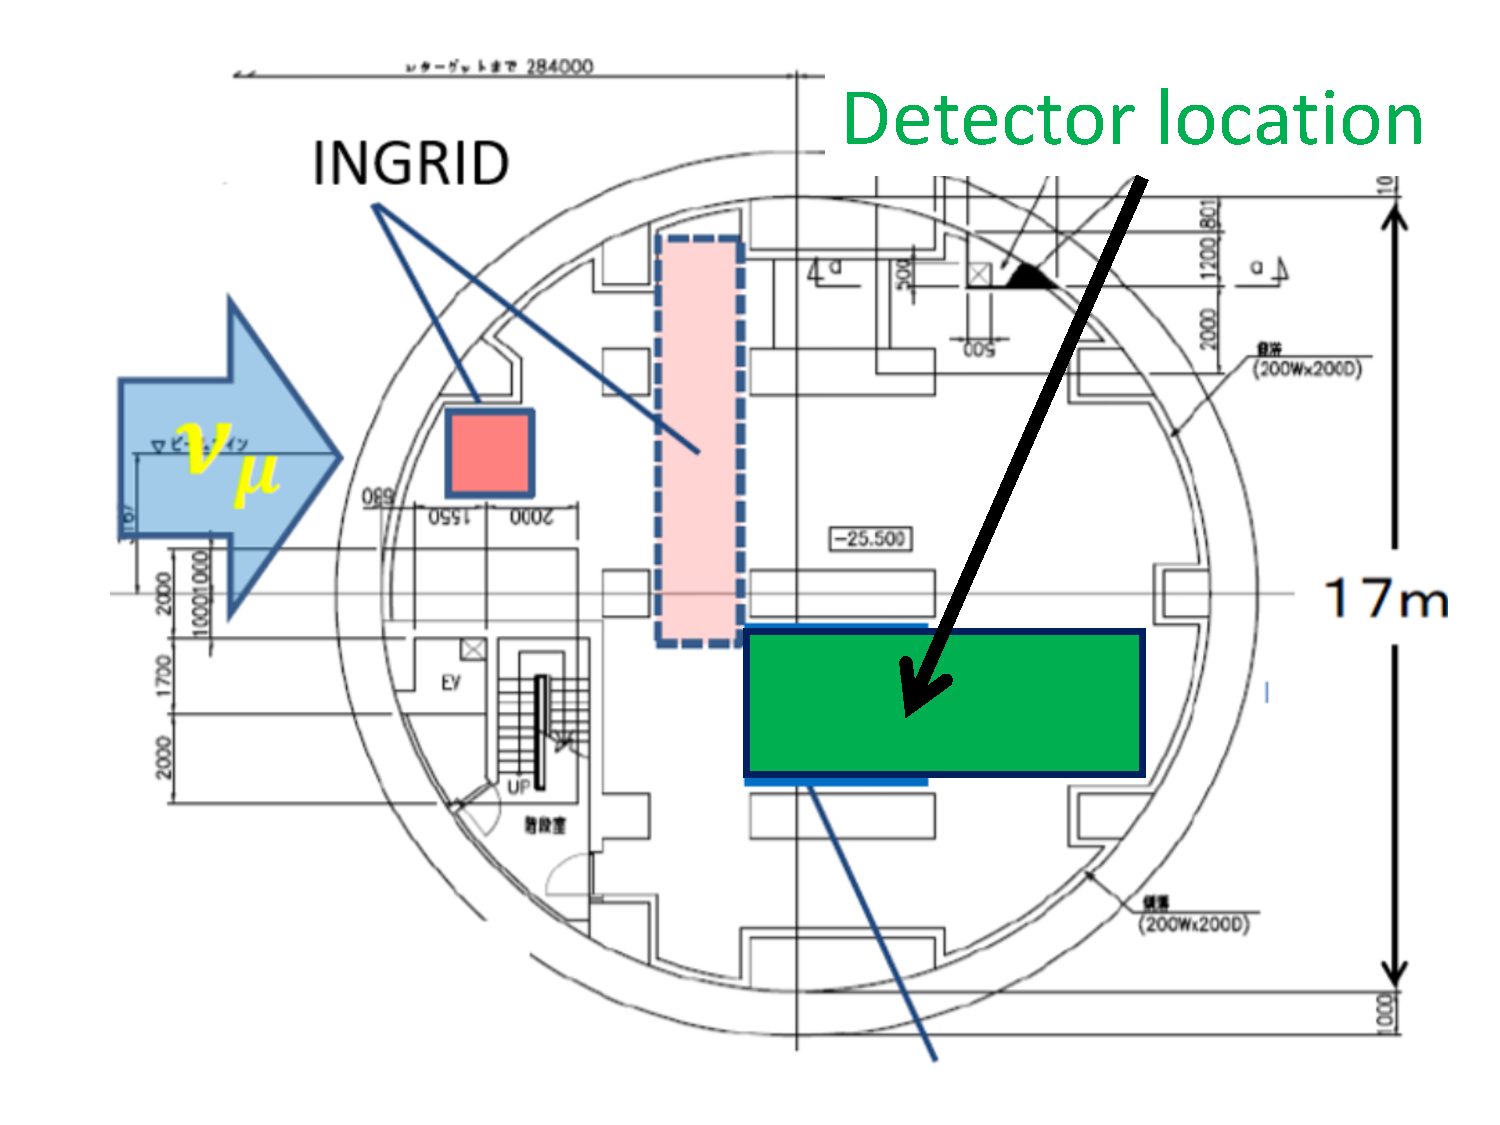
\includegraphics[width=0.7\textwidth]{figs/detector_position_b2.pdf}
  \caption{Candidate detector position in the B2 floor of the T2K near detector hall.}
  \label{fig:detector_position_b2}
  \end{center}
\end{figure}

\begin{figure}%[htbp]
  \begin{center}
  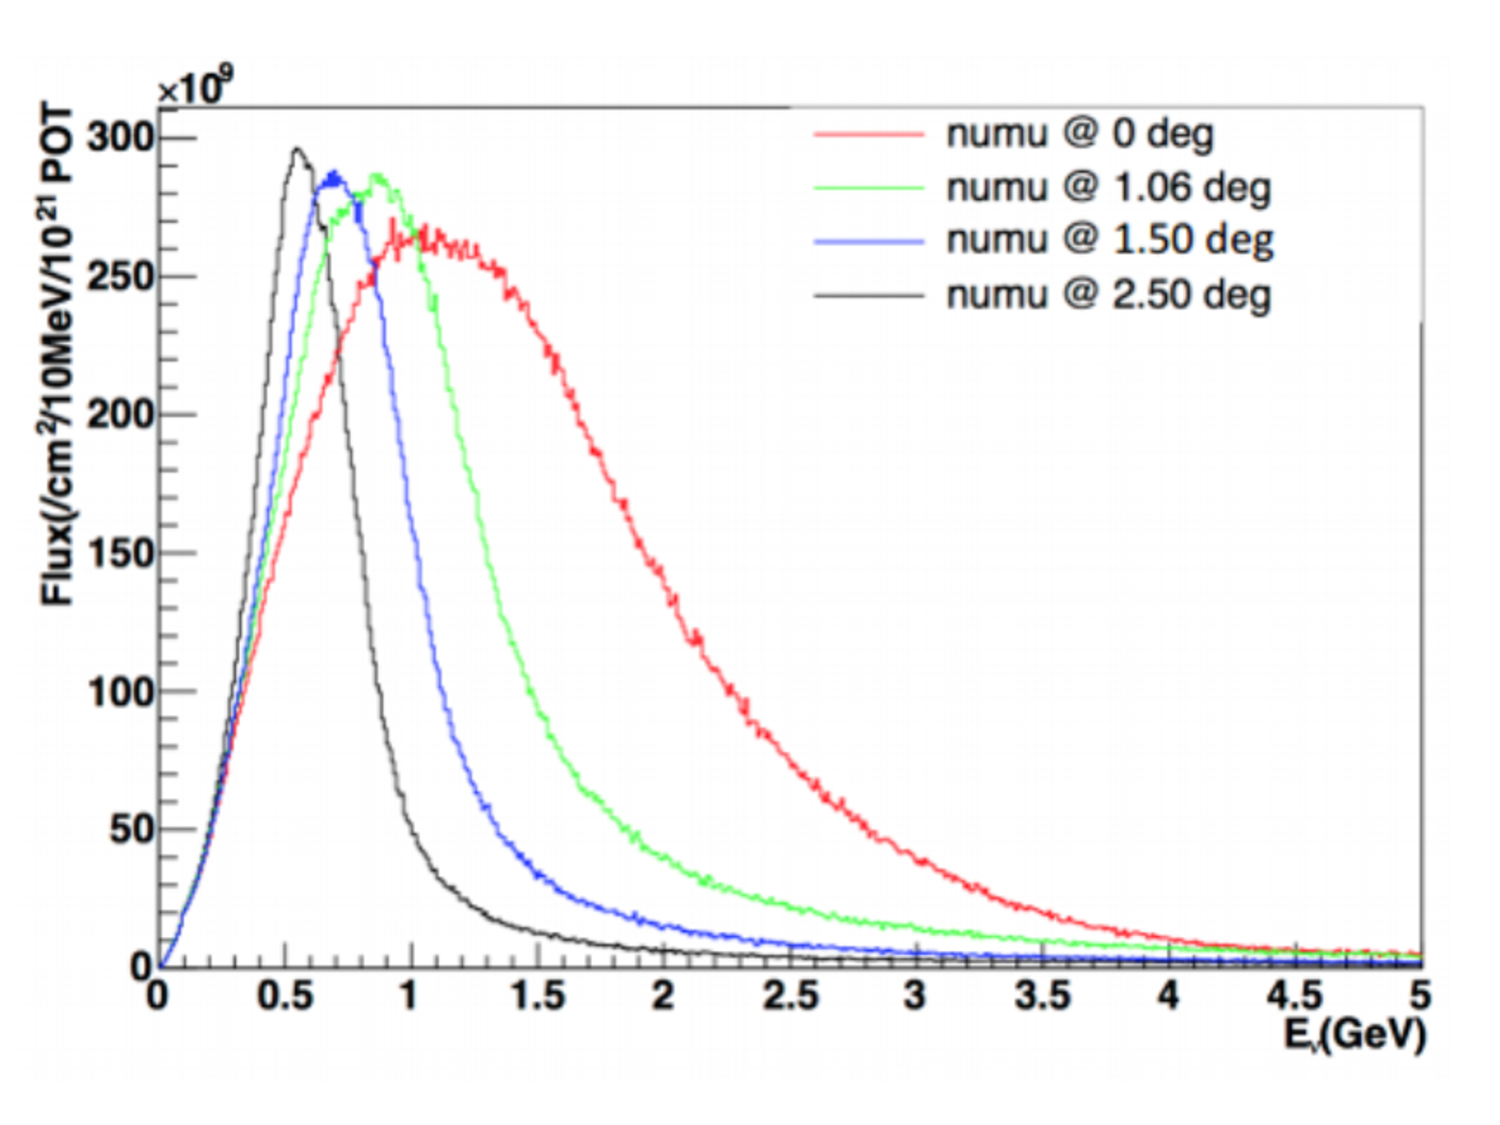
\includegraphics[width=0.6\textwidth]{figs/nu_flux_b2.pdf}
  \caption{Neutrino energy spectrum at the candidate experimental site (blue). 
  The spectra at the ND280 site (black) and INGRID center module (red) are also shown.}
  \label{fig:nu_flux_b2}
  \end{center}
\end{figure}


\subsection{Staging approarch}
We are adopting a staging approach to provide the outcomes in a timely manner.
As a prototype measurement, we had constructed one WAGASCI module and started neutrino beam measurement in SS floor of the near detector hall from October 2016.
In the prototype measurement, WAGASCI module is placed in front of the existing T2K on-axis near detector, INGRID as shown in Fig. \ref{fig:SS_config}.
Here, the INGRID modules are used as downstream MRDs.
The preliminary results from the prototype measurements are summarized in Sec. \ref{sec:achievements}.

\begin{figure}%[htbp]
  \begin{center}
  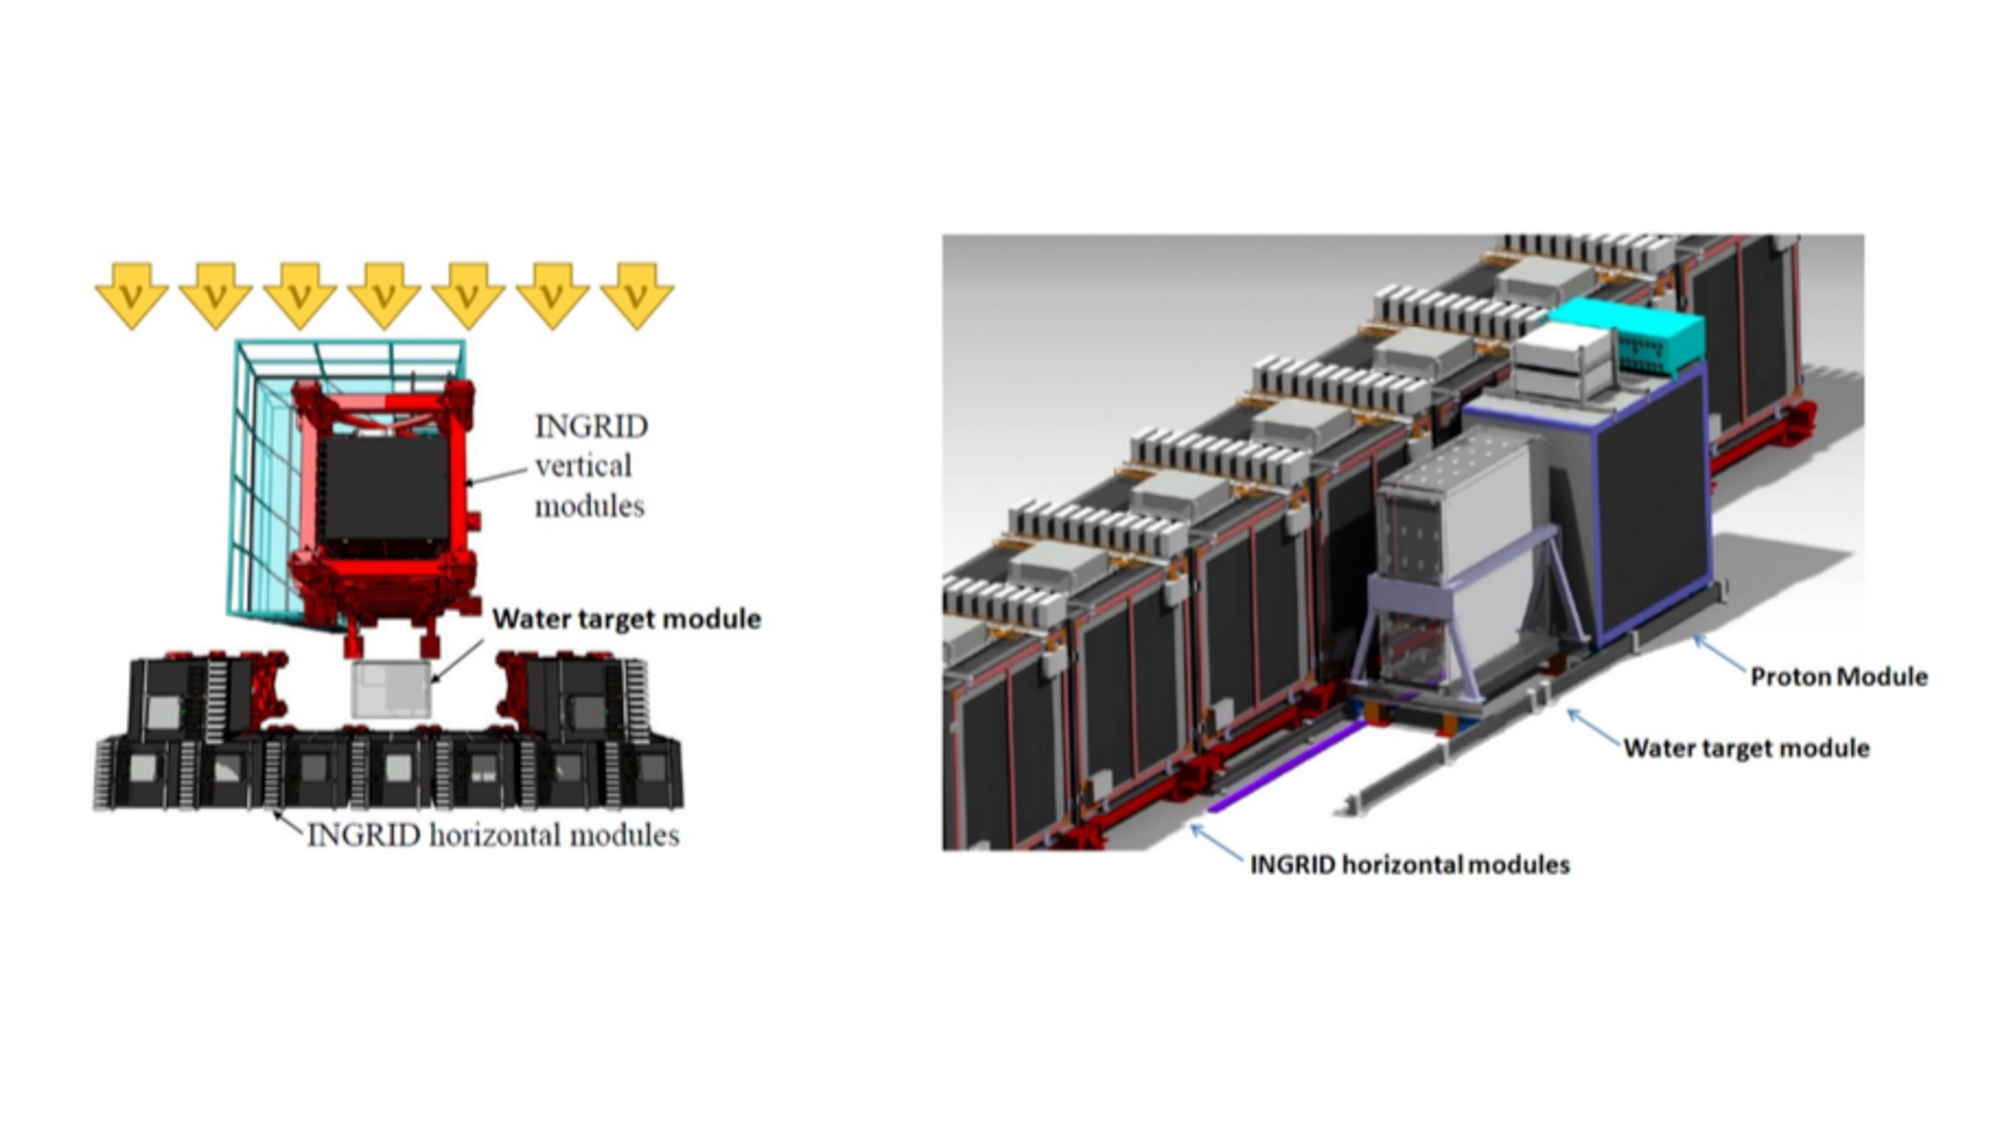
\includegraphics[width=1.0\textwidth]{figs/SS_config.pdf}
  \caption{Detector configuration of the prototype measurement.}
  \label{fig:SS_config}
  \end{center}
\end{figure}


A rehearsal of the neutrino beam measurement in B2 floor of the near detector hall
will be performed  from October 2017 to March 2018.
In the rehearsal, one WAGASCI module is placed between the INGRID standard module and INGRID Proton module as shown in Fig. \ref{fig:B2_test_config}.
Here, the INGRID modules are used as a downstream MRD and another neutrino target detector.
The INGRID modules are the ones which are not used for the T2K neutrino beam monitoring,
and will not cause any effect on the T2K data taking.
We had submitted a proposal to T2K collaboration, and got an approval to use these modules for the rehearsal.

\begin{figure}%[htbp]
  \begin{center}
  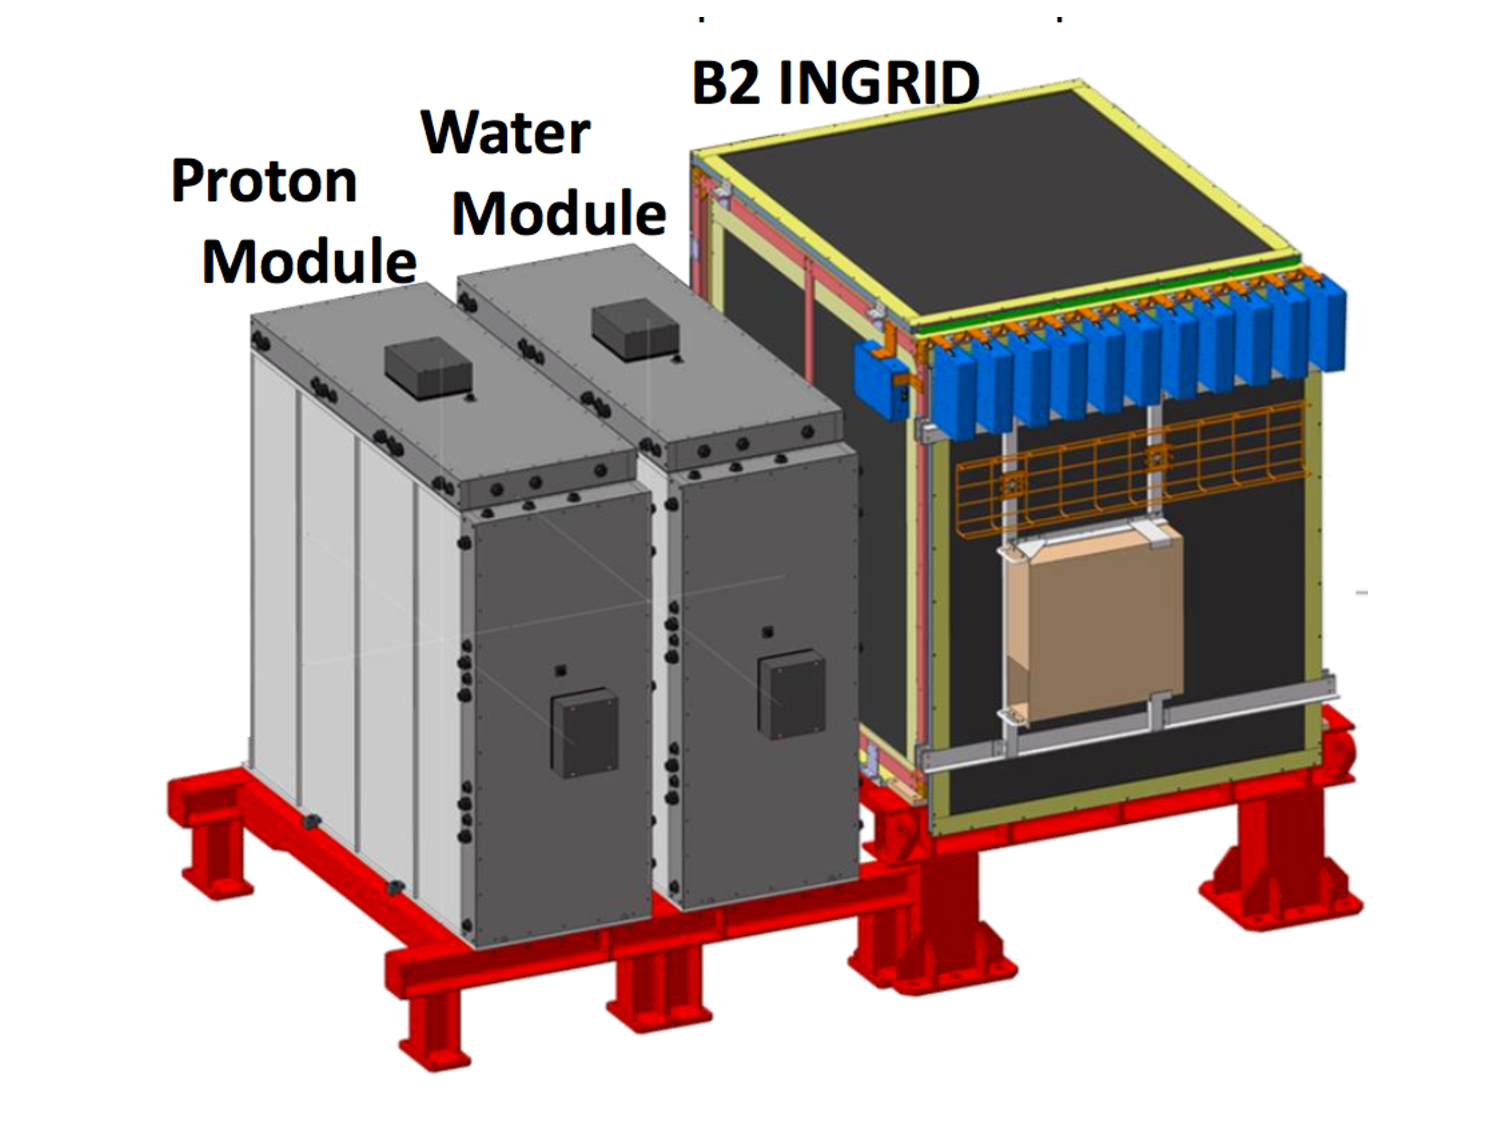
\includegraphics[width=0.7\textwidth]{figs/B2_test_config.pdf}
  \caption{Detector configuration of the prototype measurement.}
  \label{fig:B2_tes_config}
  \end{center}
\end{figure}

Finally, we will install two WAGASCI modules, two side MRD modules and Baby MIND in B2 floor of the near detector hall and will complete the detector commissioning by the end of March 2018, and will start neutrino beam measurement with the baseline configuration from April 2018.

\section{Goals of the test experiment}

\section{Schedule}
In 2016 (achieved),
\begin{itemize}
\item XXX: 1st WAGASCI module construction
\item XXX: Installation of 1st WAGASCI module to SS floor of the near detector hall.
\item XXX: Commissioning of 1st WAGASCI module
\item October: start the prototype measurement in SS floor of the near detector hall.
\end{itemize}
In 2017,
\begin{itemize}
\item XXX: 2nd WAGASCI module construction
\item XXX: Commissioning of 2nd WAGASCI module
\item October: start the rehearsal with the existing INGRID modules in B2 floor of the near detector hall.
\item XXX: Side-MRD modules construction
\item XXX: Baby-MIND plan
\end{itemize}
In 2018,
\begin{itemize}
\item XXX: Installation of Side-MRD modules and Baby-MIND.
\item XXX: Commissioning with the baseline configuration.
\item April: start neutrino beam measurement with the baseline configuration in B2 floor of the near detector hall.
\end{itemize}


Schedule in 2017 and 2018 is summarized in Fig. \ref{fig:schedule_2017_2018}.
\section{Requests}
\subsection{Beam condition and beam time}
The test experiment can run parasitically with T2K,
therefore we request no dedicated beam time nor beam condition.


We request XXX POT of $\nu$ (and anti-$\nu$) beam data for the test experiment.
In order to achieve the goals discussed in Sec. \ref{sec:goals}, we would like to use the B2 floor of the near detector hall of the J-PARC neutrino beam-line as a test facility of the neutrino beam.

\subsection{Request of equipment}
We would like to request to use the following equipments by the end of the test experiment.
\begin{itemize}
\item Working space in the neutrino assembly (NA) building for detector construction and commissioning
\item Experimental space for the detectors and the electronics/DAQ in the B2 floor of the near detector hall
\item Electricity (~XXkW) for the electronics/DAQ and the magnet modules of Baby MIND
\item Beam timing signal and spill information
\item Network connection
\end{itemize}
The infrastructure for all these is already existing.
Equipment such as the detector itself will be covered by external funds.
\section{Summary}


%\section{}
%\subsection{}



\end{document}  